\documentclass[envcountsame]{llcns2e/llncs}
\usepackage{url}
\usepackage{amsmath,amsfonts}
\usepackage{bbm}
\usepackage{algorithm,algorithmicx}
\usepackage{graphicx}
\usepackage{bm}
\usepackage{bbm}
\usepackage[titletoc]{appendix}
\usepackage{algpseudocode}
\usepackage{pifont}
\usepackage[FIGTOPCAP]{subfigure}

\newtheorem{fact}{Fact}
\DeclareMathOperator{\dom}{dom}
\DeclareMathOperator{\proj}{proj}
\DeclareMathOperator{\prox}{prox}

\title{\hrule\hrule\bigskip\bigskip A simple and efficient algorithm for computing approximate
  Nash equilibria in two-person zero-sum games with imcomplete
  information}
\author{Elvis DOHMATOB\\\email{elvis.dohmatob@inria.fr}}
\institute{
Parietal team, Inria Saclay Ile-de-France, Saclay, France
}


% The \author macro works with any number of authors. There are two commands
% used to separate the names and addresses of multiple authors: \And and \AND.
%
% Using \And between authors leaves it to \LaTeX{} to determine where to break
% the lines. Using \AND forces a linebreak at that point. So, if \LaTeX{}
% puts 3 of 4 authors names on the first line, and the last on the second
% line, try using \AND instead of \And before the third author name.


%\nipsfinalcopy % Uncomment for camera-ready version
%%%%%%%%%%%%%%%%%%%%%%%%%%%%%%%%%%%%%%%%%%%%%%%%%%%%%%%%%%%%%%%%%%%%%%%%%%%%%%%

\begin{document}


\maketitle

\begin{abstract}
We present a simple primal-dual algorithm for computing approximate
Nash equilibria in two-person zero-sum sequential games with
imcomplete information and perfect recall (like Texas Hold'em
Poker) based on the notion of enlarged subgradients.
Our algorithm only performs basic iterations (i.e iterations
involving no calls to external first-order oracles, etc.) and is
applicable to a broad class of two-person zero-sum games including
simultaneous games and sequential games with imcomplete information
and perfect recall. The number of iterations need to produce a Nash
equilibrium with a given precision is inversely proportion to the
precision. The applicability to the latter kind of games is thanks to
the sequence-form representation \cite{koller1992complexity}. As
proof-of-concept, we apply our algorithm to solve Kuhn 3-card Poker.
\end{abstract}

\textbf{keywords}: sequential game; imcomplete information; perfect
recall; sequence-form; approximate Nash equilibrium; primal-dual
algoithm; convex-optimization; enlarged subgradient

\section{Introduction}
\label{sec:intro}
A game-theoretic approach to playing games strategically optimally
consists in computing Nash-equilibria (infact, approximations thereof)
offline, and playing one's part of the equilibrium online. This
technique is the driving-force behind solution concepts like CFR
(\textbf{TODO: add Z.'s ref first!!!}) \cite{lanctot2009monte},
$\text{CFR}^{+}$ \textbf{TODO: add ref!!!}, and other variants, which
have recently had profound success in Poker. However, solving games
for equilibria remains a mathematical and computational challenge,
especially in sequential games with imperfect information. This paper
proposes a simple and fast algorithm for solving for such equilibria
approximately, in a sense which will be made clear shortly.

\subsection{Notation and terminology}
\paragraph{\textbf{General notions.}}
Let $m$ and $n$ be positive integers.
$\mathbb{R}^{n}_+ := \{z \in \mathbb{R}^{n}\text{ }|\text{ } z \geq
0\}$ is the nonnegative $n$-dimensional \textit{orthant}.  The
components of a vector $z \in \mathbb{R}^n$ will be denoted $z_0$,
$z_1$, ..., $z_{n-1}$ (indexing begins from $0$, and not $1$). The
notation ``$z \ge 0$'' means that all the components of $z$ are
nonnegative. For a vector $z = (z_0, z_1, ..., z_{n-1}) \in
\mathbb{R}^n$, %% $\|z\|$ denotes the $2$-\textit{norm} of $z$ defined
%% by $\|z\| := \sqrt{z^Tz} = \sqrt{\sum_{j=0}^{n - 1}{z_j^2}}$.
$(z)_+:=\text{max}(0, z) \in \mathbb{R}^{n}_+$ is the point-wise
maximum of $z$ with $0$.
%% For example, $((-2, \pi))_+ = (max(-2, 0),
%% max(\pi, 0)) = (0, \pi)$.
The operator $(.)_+$ is the well-known
(multi-dimensional) \textit{ramp} function.
$\mathbb{R}^{m \times n}$ denotes the space of all $m$-by-$n$ real
matrices, $I_m$ denotes the $m$-by-$m$ identity matrix, and $0_{m,n}$
denotes the $m$-by-$n$ matrix of zeros.
Given a matrix $A \in \mathbb{R}^{m \times n}$, its \textit{spectral
  norm}, denoted $\|A\|$, is
 defined to be the largest \textit{singular value} of $A$, i.e the
 largest \textit{eigenvalue} of $A^TA$ (or equivalently, of $AA^T$).

\paragraph{\textbf{Convex analysis.}}
Given a subset $C$ of $\mathbb{R}^n$,
$i_C$ denotes its \textit{indicator function} defined by
\begin{eqnarray}
  i_C(x) = 0, \text{ if } x \in C;\hspace{.3em} i_c(x) = \infty\text{
    otherwise.}
\end{eqnarray}

Let $f : \mathbb{R}^n \rightarrow (-\infty, +\infty]$ be a convex
  function.
The \textit{effective domain} of $f$, denoted $\dom(f)$ is defined as
\begin{eqnarray}
  \dom(f) := \{x \in \mathbb{R}^n | f(x) < +\infty\}.
\end{eqnarray}
 If $\dom(f) \ne \emptyset$ then we say $f$ is \textit{proper}.
%% \textit{proper convex lower semi-continous function}
%% (\textit{p.c.l.s.c} for short).
%% The \textit{Fenchel-Legendre transform} of $f$ is the function $f^*:
%% \mathbb{R}^n \rightarrow (-\infty, +\infty]$ defined by $f^*(x) \equiv
%%   \underset{z \in \mathbb{R}^n}{\text{max}}\text{}z^Tx - f(z)$.
The \textit{subgradient} of $f$ is the set-valued function
\begin{eqnarray}
\partial f: X \rightarrow 2^{\mathbb{R}^n}, \hspace{.5em} x \mapsto
\{h\in \mathbb{R}^n | f(z)  \ge f(x) + \langle h, z - x\rangle \forall
z \in X\}.
\end{eqnarray}
Of course $\partial f(x)$ reduces to the singleton $\{\nabla f(x)\}$
in case $f$ is differentiable at $x$. Given $\tau > 0$, the function
\begin{eqnarray}
  \prox_{\tau f}: \mathbb{R}^n \rightarrow \mathbb{R}^n,\hspace{.5em}x
  \mapsto \underset{z \in \mathbb{R}^n}{\text{min }}\frac{1}{2}\|z
  - x\|^2 + \tau f(z),
\end{eqnarray}

is called the \textit{proximal operator} of $f$ at rank $\tau$.
The interested reader should refer to
\cite{rockafellar1997convex,combettes2011proximal} for a more
elaborate exposition of convex-analytical concepts and their use in
optimization.

\subsection{Statement of the problem}
The sequence-form for two-person zero-sum games was introduced in
\cite{koller1992complexity}, and the theory was further developed in
\cite{koller1994fast,von1996efficient,vonequilibrium}, where it was
established that for sequential two-person zero-sum games with
imcomplete information and perfect recall, there exist sparse matrices
$A \in \mathbb{R}^{n_1
  \times n_2}$, $E_1 \in \mathbb{R}^{l_1 \times n_1}$, $E_2 \in
\mathbb{R}^{l_2 \times n_2}$, and vectors $e_1 \in \mathbb{R}^{l_1},
e_2 \in \mathbb{R}^{l_2}$ such that $n_1$, $n_2$, $l_1$, and $l_2$ are
all linear in the size of the game tree (number of states in the game)
and such that Nash equilibria correspond to pairs $(x, y)$ of
\textit{realization plans} which solve the primal LCP
\begin{equation}
  \begin{aligned}
     \text{minimize }e_1^Tp, \hspace{.5em}\text{ subject to }(y,p) \in
     \mathbb{R}^{n_2} \times \mathbb{R}^{l_1}, -Ay +
    E_1^Tp \geq 0, E_2y = e_2, y \ge 0.
  \end{aligned}
  \label{eq:primal_pb}
\end{equation}

and the dual LCP
\begin{equation}
  \begin{aligned}
    \text{maximize}-e_2^Tq,\hspace{.5em}\text{subject to }(y,q) \in
    \mathbb{R}^{n_1} \times \mathbb{R}^{l_2}, A^Tx + E_2^Tq \geq 0,
    E_1x = e_1, x \ge 0.
  \end{aligned}
  \label{eq:dual_pb}
\end{equation}
The vectors $p = (p_0, p_1, ..., p_{l_2 - 1}) \in \mathbb{R}^{l_2}$
and $q = (q_0, q_1, ..., q_{l_1 - 1}) \in \mathbb{R}^{l_1}$ are dual
variables. 
$A$ is the \textit{payoff matrix} and each $E_k$ is a matrix whose
entries are $-1$, $0$ or $1$, and each $e_k$ is a vector of the form
$[1, 0, ..., 0]$. In this so-called \textit{sequence-form}
representation, the strategy profile of player $k$ is the polyhedron
\begin{equation}
  Q_k := \{z \in \mathbb{R}^{n_k}_+ |\text{ }E_kz = e_k\}.
\label{eq:polyhedron}
\end{equation}
Note that $p^Te_1 = p_0$ and $q^Te_2 = q_0$ by definition of $e_1$ and
$e_2$. At a feasible point $(y, p, x, q)$, the \textit{primal-dual gap}
$\mathcal{G}(y, p, x, q)$ of these primal-dual pair of LCPs is given
by\footnote{The inequality being due to \textit{weak duality}.}
\begin{equation}
  0 \le \mathcal{G}(y, p, x, q) := p_0 - (-q_0) = p_0 + q_0.
  \label{eq:dgap}
\end{equation}

%\subsection{Characterization of equilibria}
It was shown (see Theorem 3.14 of \cite{vonequilibrium}) that a pair
$(x, y) \in Q_1 \times Q_2$ of realization plans is a solution to the
LCPs \eqref{eq:primal_pb} and \eqref{eq:dual_pb} (i.e is a Nash
equilibrium for the game)  if and only if there exist vectors $p$ and
$q$ such that
\begin{equation}
\hspace{.25em} -Ay + E_1^Tp \ge 0, \hspace{.5em}A^Tx + E_2^Tq \ge
0, \hspace{.25em} x^T(-Ay + E_1^Tp) = 0, \hspace{.25em} y^T(A^Tx +
E_2^Tq) = 0.
\label{eq:feasibility}
\end{equation}

Moreover, at equilibria, \textit{strong duality} holds and the value
of the game equals $p_0 = -q_0$, i.e the primal-dual gap
$\mathcal{G}(y, p, x, q)$ defined in \eqref{eq:dgap} vanishes at
equilibria.


%% As usual, the ``minimax'' notation in problem \eqref{eq:primal_pb} means that a pair $(x^*, y^*) \in Q_1 \times Q_2$ is a solution if (and only if)
%% \begin{equation}
%%   x^TAy^* \le x^TAy \le {x^*}^TAy, \forall (x, y) \in Q_1 \times Q_2
%% \label{eq:nash_ineq}
%% \end{equation}
%% Such pairs $(x^*, y^*)$ correspond to the Nash equilibria of the game, and ${x^*}^TAy^*$ is the \textit{value}
%% \footnote{This value is the same for every equilibrium pair $(x^*, y^*)$.} of the game.

\begin{remark}  
It should be noted that for the the class of games considered here (sequential games with imcomplete information), the LCPs \eqref{eq:primal_pb} and \eqref{eq:dual_pb} are exceedingly larger than what state-of-the-art LCP solvers can handle. See \cite{hoda2010smoothing}.
\end{remark}

Solving the LCPs \eqref{eq:primal_pb} and \eqref{eq:dual_pb} exactly is impossible in practice \textbf{Cite Koller!!!}, and such a precision doesn't have any fundamental advantage. Instead, it is customary compute so-called Nash $\epsilon$-equlibria.

\begin{definition}[\textbf{Nash $\epsilon$-equilibria}]
Given $\epsilon > 0$, a Nash $\epsilon$-equilibrium is
a pair $(x^*, y^*)$ of realization plans such that there exists dual
vectors $p^*$ and $q^*$ for problems \eqref{eq:primal_pb} and
\eqref{eq:dual_pb} such that the primal-dual gap at $(y^*, p^*, x^*, q^*)$
doesn't exceed $\epsilon$. That is,

\begin{equation}
  0 \le \mathcal{G}(y^*, p^*, x^*, q^*) \le \epsilon.
\label{eq:approx_pb}
\end{equation}
\label{thm:approx_nash}
\end{definition}

\subsection{Our contribution}
We develop a $\mathcal{O}(1/\text{min}(\rho,\epsilon))$ primal-dual
algorithm (Algorithm \ref{Tab:algo}) for computing Nash $(\rho,
  \epsilon$)-equilibria (in a sense to be made clear later in
  Definition \ref{thm:cool_notion}) for
  sequential two-person zero-sum games with imcomplete information and
  perfect recall.

\section{Related work}
\label{sec:related_work}
\textbf{TODO: add note about interior-point methods!!!}

We present a selection of algorithms that is representative of the
efforts that have been made in the literature to compute Nash
$\epsilon$-equilibria for two-person zero-sum games with imcomplete
information like Texas Hold'em Poker, etc.


In \cite{hoda2010smoothing}, a nested iterative procedure using the
Excessive Gap Technique (EGT) \cite{nesterov2005excessive} was used to
to solve the LCPs \eqref{eq:primal_pb} and \eqref{eq:dual_pb} in the
following equivalent saddle-point form


\begin{equation}
  \underset{y \in Q_2}{\text{minimize}}\text{ }\underset{x \in
    Q_1}{\text{maximize}}\text{ }x^TAy.
  \label{eq:gilpin}
\end{equation}
The authors reported a $\mathcal{O}(1/\epsilon)$ convergence rate
(which derives from the general EGT theory) for the outer-most
iteration loop, though the cost of an iteration is presumably heavy
since it entails computing a $softmax$ at each iteration.


\cite{gilpinfirst} proposed a modified verson of the technqiues in
\cite{hoda2010smoothing} and  proved a $\mathcal{O}\left(\left(\|A\| /
\delta\right) ln\left(1 / \epsilon\right)\right)$ convergence rate in
terms of the number of calls made to a first-order oracle (for
example, Nesterov's optimal gradient \cite{nesterov1983}). Here
$\delta = \delta(A, E_1, E_2, e_1, e_2)$ is a certain
\textit{condition number} for the game. It should be noted however that
\begin{itemize}
\item[--] though \cite{gilpinfirst} proved that we always have $\delta
  > 0$, this constant can be arbitrarily small; and most importantly,
\item[--] the reported linear convergence rate is not in terms of
  basic operations (addition, multiplication, matvec, clipping, etc.),
  but in terms of the number of calls to a first-order oracle. Of
  course, the existence of a linear algorithm for solving
  \eqref{eq:gilpin} is improbable, as the usual strong-convexity
  conditions are absent.

\end{itemize}

%% It should be noted that the EGT and its precursors have had
%% considerable success in the signal processing communities, as can
%% be seen in \cite{NestaCandès, eduard, etc.} and the references
%% therein.


The primal-dual algorithm first developed in \cite{chambolle2010} was
proposed \cite{chambolle2014ergodic} in to solve matrix games on
simplexes. It should be stressed that such matrix games are
considerably simpler than the games considered here. Indeed, the
authors in \cite{chambolle2014ergodic} use the fact that computing the
euclidean projection of a point unto a simplex can be done in linear
time as in \cite{duchi2008efficient}. In contrast, no such efficient
algorithm is known nor is likely to exist for the polyhedra $Q_k$
defined in \eqref{eq:polyhedron}, the strategy profiles for players in
the games considered here. It should however be noted that such this
projection can still be done iteratively using, for example, the
algorithm in proposition 4.2 of \cite{combettes2010dualization}%%  or any
%% CQ algorithm (since this projection sub-problem, is, in fact a
%% \textit{split-feasibility problem}), for example
. Unfortunately, as
with any nested iterative scheme, one would have to solve this
sub-problem with finer and finer precision.


Sampling techniques like the CFR (CounterFactual Regret minimization)
and its many variants
\cite{MartinZinkevichNIPS2007,lanctot2009monte,Bowling09012015} have
also become state-of-the-art.


\section{Reformulation as a Generalized Saddle-point Problem (GSP)}
\label{sec:gsp}
One cannot directly attack the LCPs \eqref{eq:primal_pb} and
\eqref{eq:dual_pb} via a traditional primal-dual algorithm
(for example \cite{chambolle2010,chambolle2014ergodic}) because
computing the euclidean projections $\proj_{Q_k}$ is very difficult
(in fact, such subproblems would have to be solved
iteratively\footnote{An ``exception to the rule'' is the case where
  the $Q_k's$ are simplexes, so that the projections can be computed
  exactly using \cite{duchi2008efficient}.}). Also,
the primal-dual gap might explode even at ``nearly feasible'' points,
leaving a primal-dual algorithm with no clear on whether progress is
being made or not. So need to way to
\begin{itemize}
\item avoid having to compute the projections $\proj_{Q_k}$,
\item have control over how far we are from the set of equilibria,
\item cope  with infinite primal-dual gaps.
\end{itemize}

In the next theorem, we show that the said LCP problems can be
conveniently written as a \textit{Generalized Saddle-point Problem
  (GSP)} in the sense of \cite{he2013accelerating}.
\begin{theorem}
Define two proper closed convex functions
  \begin{eqnarray}
    \left.
    \begin{aligned}
      g_1: \mathbb{R}^{n_2} &\times \mathbb{R}^{l_1} \rightarrow
      (-\infty, +\infty], \hspace{1em} g_1(y, p) :=
        i_{\mathbb{R}^{n_2}_+}(y) + e_1^Tp\\
        g_2: \mathbb{R}^{n_1} &\times \mathbb{R}^{l_2} \rightarrow
        (-\infty, +\infty],\hspace{1em} g_2(x, q) :=
          i_{\mathbb{R}^{n_1}_+}(x) + e_2^Tq.
    \end{aligned}
    \right\}
    \label{eq:things}
  \end{eqnarray}

Also, define two bilinear forms $\Psi_1$, $\Psi_2: \mathbb{R}^{n_2}
\times \mathbb{R}^{l_1} \times \mathbb{R}^{n_1} \times
\mathbb{R}^{l_2} \rightarrow \mathbb{R}$ by letting
  \begin{equation}
      K :=
      \left[
        \begin{array}{cc}
          A & -E_1^T \\
          E_2 & 0_{l_2, l_1}
        \end{array}
        \right],\hspace{.5em}
    \Psi_1(y, p, x, q)
    := \begin{bmatrix}x\\q\end{bmatrix}^TK\begin{bmatrix}y\\p\end{bmatrix}, \hspace{.5em}
      \Psi_2(y, p, x, q) := -\Psi_1(y, p, x, q).
\end{equation}

Finally, define the functions $\hat{\Psi}_1$, $\hat{\Psi}_2:
\mathbb{R}^{n_2} \times \mathbb{R}^{l_1} \times \mathbb{R}^{n_1}
\times \mathbb{R}^{l_2} \rightarrow (-\infty, +\infty]$ by
\begin{eqnarray}
  \left.
  \begin{aligned}
    \hat{\Psi}_1(y, p, x, q) &:=
    \Psi_1(y, p, x, q)+ g_1(y, p) \text{ if }y \ge 0, \hat{\Psi}_1(y,
    p, x, q) := \infty \text{ else}\\
    \hat{\Psi}_2(y, p, x, q) &:= \Psi_2(y, p, x, q)+ g_2(x, q) \text{ if
    }x \ge 0, \hat{\Psi}_2(y,p, x, q) := \infty \text{ else}.
  \end{aligned}
  \right\}
\end{eqnarray}

Define the sets $S_1 := \mathbb{R}^{n_2}_+ \times \mathbb{R}^{l_1}$ and $S_2 :=
\mathbb{R}^{n_1}_+ \times \mathbb{R}^{l_2}$ and consider the
GSP($\Psi_1$, $\Psi_2$, $g_1$, $g_2$): Find $(y^*,p^*, x^*, q^*) \in
S_1 \times S_2$ such that
\begin{eqnarray}
  \left.
  \begin{aligned}
    \hat{\Psi}_1(y^*, p^*, x^*, q^*) \le \hat{\Psi}_1(y, &p, x^*,
    q^*),\hspace{.5em} \hspace{.5em}\hat{\Psi}_2(y^*, p^*, x^*, q^*)
    \le \hat{\Psi}_2(y^*, p^*, x, q)\\
    &\forall (y,p, x, q) \in S_1 \times S_2.
  \end{aligned}
  \right\}
  \label{eq:unconstrained_pb}
\end{eqnarray}
\label{thm:pd}

Then a quadruplet $(y^*,p^*, x^*, q^*) \in \mathbb{R}^{n_2}
  \times \mathbb{R}^{l_1} \times \mathbb{R}^{n_1} \times
  \mathbb{R}^{l_2}$ solves the Nash equilibrium LCPs
  \eqref{eq:primal_pb} and \eqref{eq:dual_pb} iff it solves
  GSP($\Psi_1$, $\Psi_2$, $g_1$, $g_2$).
  \label{thm:pd}
\end{theorem}

\begin{proof}
Note that $\dom(g_1) = S_1$ and $\dom(g_2) = S_2$ and observe that the
equilibria of the LCPs \eqref{eq:primal_pb}, \eqref{eq:dual_pb}, and
the equilibria of GSP($\Psi_1$, $\Psi_2$, $g_1$, $g_2$) are contained
in $S_1 \times S_2$, it suffices to show that at any point $(y, p, x,
q) \in S_1 \times S_2$, the primal-dual gap between the primal
LCP \eqref{eq:primal_pb} and the dual LCP \eqref{eq:dual_pb} equals
the primal-dual gap of GSP($\Psi_1$, $\Psi_2$, $g_1$, $g_2$).
Indeed, the unconstrained objective in \eqref{eq:primal_pb}, say
$a(x,y)$, can be computed as
\begin{eqnarray*}
  \begin{aligned}
    a(y,p) &= e_1^Tp +
    i_{\mathbb{R}^{n_2}_+}(y) + i_{\mathbb{R}^{n_1}_+}(-Ay + E_1^Tp) +
    i_{\{0\}}(E_2y - e_2)\\
    &= g_1(y,p) +
    i_{\mathbb{R}^{n_1}_+}(-Ay + E_1^Tp) + i_{\{0\}}(E_2y - e_2)\\
    &= g_1(y,p) + \underset{x' \geq
      0}{\text{max}}\text{ }x'^T(Ay - E_1^Tp) +
    \underset{q'}{\text{max}}\text{ }q'^T(E_2y - e_2)\\
    &= g_1(y,p) + \underset{x',
      q'}{\text{max}}\text{ }x'^TAy - x^TE_1^Tp + q'^TE_2y -
    (i_{\mathbb{R}^{n_1}_+}(x') + e_2^Tq)\\
    &= g_1(y,p)
      - \underset{x',q'}{\text{min}}\text{ }\Psi_2(y, p, x', q') + g_2(x',
      q') = g_1(y,p) -\phi_2(y,p),
  \end{aligned}
  \label{eq:a}
\end{eqnarray*}

where $-\infty \le \phi_2(y, p) := \underset{x',q'}{\text{min}}\text{
}\hat{\Psi}_2(y, p, x', q') < +\infty$.
Similarly, the unconstrained objective, say
$b(x, q)$, in the dual LCP \eqref{eq:dual_pb} writes
\begin{eqnarray*}
  \begin{aligned}
 b(x, q) &= 
 -i_{\mathbb{R}^{n_1}_+}(x) - i_{\mathbb{R}^{n_2}_+}(A^Tx+E_2^Tq) -
 i_{\{0\}}(e_1 - E_1x)\\
    &= -g_2(x, q) + \underset{y' \geq
   0}{\text{min}}\text{ }y'^T(A^Tx + E_2^Tq) +
 \underset{p'}{\text{min}}\text{ }p'^T(e_1-E_1x)\\
    &= -g_2(x, q)
 +\underset{y',p'}{\text{max}}\text{ }\Psi_1(y', p', x, q) +
 g_1(y', p') = -g_2(x, q) + \phi_1(x, q),
   \end{aligned}
\end{eqnarray*}
where $-\infty \le \phi_1(x, q) :=
\underset{y',p'}{\text{min}}\text{ }\hat{\Psi}_1(y', p', x, q) < +\infty$.
Thus, one can compute the primal-dual gap between primal LCP
\eqref{eq:primal_pb} and dual LCP \eqref{eq:dual_pb} at $(y, p, x, q)$ as
\begin{eqnarray*}
  \begin{split}
  a(y, p) - b(x, q) &= g_1(y, p) - \phi_2(y, p) + g_2(x, q) - \phi_1(x,
  q) \\
  &= \Psi_1(y, p, x, q) +  g_1(y, p) - \phi_2(y, p) + \Psi_2(y, p, x,
  q) + g_2(x, q) - \phi_1(x, q)\\
  &= \hat{\Psi}_1(y, p, x, q) + \hat{\Psi}_2(y, p, x, q) - \phi_1(x,
  q) - \phi_2(y, p)\\
  &= \text{primal-dual gap of GSP}(\Psi_1, \Psi_2,
  g_1, g_2) \text{ at }(y, p, x, q),
  \end{split}
\end{eqnarray*}
where the second equality follows from the fact that $\Psi_1 + \Psi_2
:= 0$.
\qed

%% For the dual-gap bound, note that $\forall (x', u', y', v') \in \mathbb{R}^{n_1}_+ \times \mathbb{R}^{l_2} \times \mathbb{R}^{n_2}_+ \times \mathbb{R}^{l_1}$, one has
%% \begin{eqnarray*}
%%   \begin{split}
%%     \underset{x \in \mathbb{R}^{n_1}, u \in \mathbb{R}^{l_2}}{max}\text{ }\begin{bmatrix}x\\u\end{bmatrix}^TK\begin{bmatrix}y'\\v'\end{bmatrix} + g_1(y', v') - g_2(x, u)
%%       &= \underset{x \in \mathbb{R}^{n_1}_+, u \in \mathbb{R}^{l_2}}{max}\text{ }x^TAy' - v'^T(E_1x - e_1) + u^T(E_2y' - e_2)\\
%%       &\ge \underset{x \in \mathbb{R}^{n_1}_+}{max}\text{ }x^TAy' - v'^T(E_1x - e_1) + \underset{u \in \mathbb{R}^{l_2}}{max}\text{ }u^T(E_2y' - e_2)\\
%%       &\ge \underset{x \in Q_1}{max}\text{ }x^TAy + \underset{u \in \mathbb{R}^{l_2}}{max}\text{ }u^T(E_2y' - e_2)
%%   \end{split}
%% \end{eqnarray*}

%% and
%% \begin{eqnarray*}
%%   \begin{split}
%%     \underset{y \in \mathbb{R}^{n_2}, v \in \mathbb{R}^{l_1}}{min}\text{ }\begin{bmatrix}x'\\u'\end{bmatrix}^TK\begin{bmatrix}y\\v\end{bmatrix} + g_1(y, v) - g_2(x', u')
%%       &= \underset{y \in \mathbb{R}^{n_2}_+, v \in \mathbb{R}^{l_1}}{min}\text{ }x'^TAy - v^T(E_1x' - e_1) + u'^T(E_2y - e_2)\\
%%       &\le \underset{y \in \mathbb{R}^{n_2}_+}{min}\text{ }x'^TAy + u'^T(E_2y - e_2) - v^T(E_1x' - e_1)
%%   \end{split}
%% \end{eqnarray*}
\end{proof}

%% The rest of this section is concerned with applying Algorithm 39 of \cite{chambolle2010} to solve problem
%% \eqref{eq:unconstrained_pb} and therefore by Theorem \ref{thm:pd}, the Nash equilibrium problems \eqref{eq:primal_pb} and \eqref{eq:dual_pb}.

% \subsection{The proposed algorithm and its $\mathcal{O}(1/\epsilon)$
% convergence}

\section{The proposed algorithm}
\label{sec:algo}
In this section we derive the algorithm which is the main object of
this manuscript.

\subsection{Relaxing the conditions for equilibrium}
Let us first introduce the notion of $\epsilon$-subgradients.

\begin{definition}[$\epsilon$-subgradient \cite{he2013accelerating}]
Given a scalar $\epsilon > 0$ and a function $f:X \subseteq \mathbb{R}^n
\rightarrow [-\infty,+\infty]$, the $\epsilon$-enlarged subgradient (or
$\epsilon$-subgradient, for short) of $f$ the set-valued function
\begin{eqnarray}
\partial_\epsilon f: X \rightarrow 2^{\mathbb{R}^n}, \hspace{.5em} x
\mapsto \{h \in \mathbb{R}^n | f(z) + \epsilon \ge f(x) + \langle h, z
- x\rangle \forall z \in X\}.
\end{eqnarray}
\end{definition}

The idea is to replace the usual necessary condition ``$0 \in \partial
f(x)$'' for the optimality of $x$ with ``$v \in \partial_\epsilon
f(x)$, for some small perturbation vector $v$''. In fact, it is easy
to see that, for each $x \in X$, $(\partial_\epsilon f(x))_{\epsilon >
  0}$ is a decreasing sequence of sets which converges to $\partial
f(x)$.

Henceforth, the notion of approximate Nash equilibria will be
understood in the following sense.

%% Since won't typically be able to compute a feasible point in $Q_1 \in
%% Q_2$ (due to the equality constraints $E_kz = e_k$), we will consider
%% an approximate equilibrium concept which takes in to account the
%% distance from the set of equilibria. Viz,

\begin{definition}[\textbf{Nash $(\rho,\epsilon)$-equilibria}
    \cite{he2013accelerating}]
Given $\rho > 0$ and $\epsilon > 0$, a Nash
$(\rho,\epsilon$)-equilibrium is a pair $(x^*, y^*)$ of realization
plans such that there exists dual vectors $p^*$ and $q^*$ and a
pertubation vector $v^*$ for which
\begin{eqnarray}
\|v^*\| \le \rho \text{ and}\hspace{.5em} v^* \in
\partial_\epsilon[\hat{\Psi}_1(., ., x^*, q^*) +
  \hat{\Psi}_2(y^*, p^*, , .)](y^*,p^*,x^*,q^*).
\end{eqnarray}
\label{thm:cool_notion}
\end{definition}

The above definition is a generalization of the notion of Nash
equilibria in the sense that
\begin{itemize}
\item Exact Nash equilibria correspond to Nash $(0^+,0^+)$-equilibria.
\item Nash $\epsilon$-equilibria (in the sense of Definition
  \ref{thm:approx_nash}) correspond to Nash $(0^+,\epsilon)$-equilibria.
\end{itemize}

%\paragraph{\textbf{Plan of attack.}}
\textbf{XXX TODO: Define the ergodic variables $\tilde{v}^a$ and
  $\tilde{\epsilon}^a$, ...}

\subsection{The algorithm proper and its convergence rate}
Consider the following algorithm for solving the GSP
\eqref{eq:unconstrained_pb}
\begin{algorithm}
\caption{Primal-dual algorithm for computing approximate Nash
  Equilbria in two-person zero-sum games with imcomplete information
  and perfect recall}
\label{Tab:algo}
\begin{algorithmic}[1]
\Require $\rho >0$, $\epsilon > 0$; $(y^{(0)},p^{(0)},x^{(0)},q^{(0)})
\in \mathbb{R}^{n_2}
  \times \mathbb{R}^{l_1} \times \mathbb{R}^{n_1} \times
  \mathbb{R}^{l_2}$.
\Ensure A Nash $(\rho, \epsilon)$-equilibrium
$(\tilde{y},\tilde{p},\tilde{x},\tilde{q}) \in S_1 \times S_2$ for
the GSP \eqref{eq:unconstrained_pb}.
\State  $\lambda \leftarrow 1/\|K\|$,
%% $y^{(0)} \leftarrow 0_{n_2}$,
%% $p^{(0)} \leftarrow 0_{l_1}$, $x^{(0)} \leftarrow 0_{n_1}$, $q^{(0)}
%% \leftarrow 0_{l_2}$,
$k \leftarrow 0$
\While{$\|\tilde{\epsilon}^{a}_k\| \ge \rho$ or $\|\tilde{v}^{a}_k\| \ge \epsilon$}
\State $y^{(k + 1)} \leftarrow (y^{(k)} - \lambda (A^Tx^{(k)} +
E_2^Tq^{(k)}))_+$
\State  \hspace{.5em}$p^{(k+1)} \leftarrow p^{(k)} -
\lambda(e_1-E_1x^{(k)})$
\State $x^{(k + 1)} \leftarrow (x^{(k)} + \lambda (Ay^{(k+1)} -
E_1^Tp^{(k+1)}))_+$
\State  \hspace{.5em}$q^{(k+1)} \leftarrow q^{(k)} +
\lambda(E_2y^{(k+1)}-e_2)$
\State $y^{(k+1)} \leftarrow y^{(k+1)} - \lambda
(A^T(x^{(k+1)}-x^{(k)}) + E_2^T(q^{(k+1)}-q^{(k)}))$
\State $p^{(k+1)} \leftarrow p^{(k+1)} + \lambda E_1(x^{(k+1)}-x^{(k)})$
\State $k \leftarrow k + 1$
\EndWhile
\end{algorithmic}
\end{algorithm}

\begin{theorem}[Ergodic $\mathcal{O}(1/k)$ convergence]
Let $d_0$ be the euclidean distance between the starting point
$(y^{(0)},p^{(0)},x^{(0)},q^{(0)})$ of Algorithm \ref{Tab:algo} and the
set of equilibria for the GSP \eqref{eq:unconstrained_pb}.
Then given any $\epsilon > 0$ and $\rho > 0$, we have the ergodic
error bounds
\begin{eqnarray}
\|\tilde{\epsilon}^{a}_k\| \le \rho\text{ and }\|\tilde{v}^{a}_k\| \le
\epsilon, \forall k \ge 2d_0\|K\|max(5d_0/\rho, 1/\epsilon).
\end{eqnarray}

Thus Algorithm \ref{Tab:algo} outputs an $(\rho,\epsilon)$-Nash
Equilibrium for the GSP \eqref{eq:unconstrained_pb}
in at most $2d_0\|K\|max(5d_0/\rho, 1/\epsilon)$ iterations.
\end{theorem}

\begin{proof}
Note that the quadruplet $(\Psi_1, \Psi_2, g_1, g_2)$ clearly satisfies
assumptions B.1, B.2, B.3, B.5, and B.6 of \cite{he2013accelerating}
with $L_{xx} = L_{yy} = 0$ and $L_{xy} = L_{yx} = \|K\|$. Now,
one easily computes the proximal operators $g_1$ and $g_2$ as
\begin{eqnarray*}
  \prox_{\lambda g_1}(y, p) \equiv ((y)_+, p - \lambda
  e_1),\hspace{.5em} \prox_{\lambda g_2}(x, q) \equiv ((x)_+, q -
  \lambda e_2).
  \end{eqnarray*}

Algorithm \ref{Tab:algo} is then obtained from \cite[Algorithm
  T-BD]{he2013accelerating}, applied on the GSP
\eqref{eq:unconstrained_pb} with the choice of parameters: $\sigma = 1
\in (0, 1]$, $\sigma_x = \sigma_y = 0 \in [0, \sigma)$,
    $\lambda_{xy} := \frac{1}{\sigma L_{xy}}\sqrt{(\sigma^2 -
        \sigma_x^2)(\sigma^2 - \sigma_y^2)} = \sigma / \|K\| =
      1/\|K\|$, and $\lambda = \lambda_{xy} \in (0,
      \lambda_{xy}]$. The convergence result follows immediately from
  \cite[Theorem 4.2]{he2013accelerating}.
  \qed
\end{proof}

\subsection{Practical considerations}
\paragraph{\textbf{Efficient computation of $Ay$ and $A^Tx$.}}
In Algorithms \ref{Tab:algo} most of the time is spent
pre-multiplying vectors by $A$ and $A^T$. For \textit{flop}-type Poker
games like \textit{Texas Hold'em} and  \textit{Rhode Island Hold'em},
$A$ (and thus $A^T$ too)  is very big (up $10^{14}$ rows and columns!)
but has a rich block-diagnoal structure which can be carefully
exploited, as was done in \cite{hoda2010smoothing}.


\begin{definition}(Kronecker product)
Let $F \in \mathbb{R}^{m \times n}$ and $B \in \mathbb{R}^{r \times
  s}$ be matrices. The kronecker product of $F$ and $B$ is defined by

\begin{equation}
F \otimes B:=\left[
\begin{array}{cccc}
F_{0,0}B & F_{0,1}B & \cdots & F_{0,n-1}B \\
F_{1,0}B & F_{1,1}B & \cdots & F_{1,n-1}B \\
\vdots & \vdots & \ddots & \vdots\\
F_{m-1,0}B & F_{m-1,1}B & \cdots & F_{m-1,n-1}B 
\end{array}\right] \in \mathbb{R}^{mr \times ns}
\end{equation}
\end{definition}

One notes that $(F \otimes B)^T = F^T \otimes B^T$.
$F \otimes B$ can be very much larger than both $F$ and $B$ in
dimensions. For example, if $r = n = r = s = 1000$, so that $F$ and
$B$ are $10^3$-by-$10^3$ matrices, then $F \otimes B$ is a
$10^6$-by-$10^6$ matrix! Fortunately, given a vector $x \in
\mathbb{R}^{rs}$ one can compute the matvec product $(F \otimes B)x$
without forming $F \otimes B$. Indeed, let $y := (F \otimes B)x$. We
rewrite the row vector $x$ as an $s$-by-$r$ matrix $X = [X_0, X_1,
  ..., X_{r-1}]$, where each column vector $X_i$ is the $i$th block of
$s$ elements of $x$ read from left to right. Similarly, rewrite $y$ as
as an $n$-by-$m$ matrix $Y = [Y_0, Y_1, ..., Y_{m-1}]$. Then one
easily verfies that $Y$ is the matrix product of the ``small''
matrices $B$, $X$, and $F^T$, i.e

\begin{equation}
  \label{eq:kron_matvec}
  Y = BXF^T
\end{equation}

Now, in Texas Hold'em for example, the payoff matrix $A$ can be
written as block-diagonal matrix whose blocks are sums of Kronecker
products of much smaller sparse matrices as follows

\begin{equation}
  A = \begin{bmatrix}F_1 \otimes B_1\hspace{10em}\\\hspace{3em}F_2
    \otimes B_2\hspace{7em}\\\hspace{6em}F_3 \otimes
    B_3\hspace{4em}\\\hspace{10em}F_4 \otimes B_4 + S \end{bmatrix}
\label{eq:factor_A}
\end{equation}
See \cite{hoda2010smoothing}. The matrices $F_i$ correspond to
sequences of moves in round $i$ which end in a \textit{fold} action,
and $S$ to the sequences which end in a \textit{showdown}. $B_i$
encodes the betting structure of round $i$, while $W$ encodes the
wind/lose/draw information determined by ranking the players' hands at
showdown. The component matrices $F_i$, $B_i$, $S$, and $W$ are small
enough to be explictly represented whereas it is infeasible to
explicitly represent A. Furthermore, the matrices $F_i$, $B_i$,
$S$, and $W$ are themselves sparse, which allows one to use the
compressed row storage data structure that only stores nonzero entries
(for example \textit{scipy.sparse.csr\_matrix}, in the Python
programming language).

Such a representation of the payoff matrix $A$ trivializes matvec
operations involving $A$ or $A^T$ (thanks to formula
\eqref{eq:kron_matvec} above, applied to their diagonal blocks and
exploiting the sparsity of these blocks themselves). Of course, one
can always write the payoff matrix $A$ of a flop-type Poker game in a
form similary to \eqref{eq:factor_A} by applying appropriate
permutations to the enumeration of the players's sequences.

\paragraph{\textbf{Computing $\|K\|$.}} Power iteration (Perron-Frobenius)...

\section{Experimantal results}
\label{sec:results}
To access the practical quality of the proposed algorithm, we
experimented it on real and simulated matrix games.

\begin{figure}[!htpb]
  \subfigure[Matrix game on simplices]{
    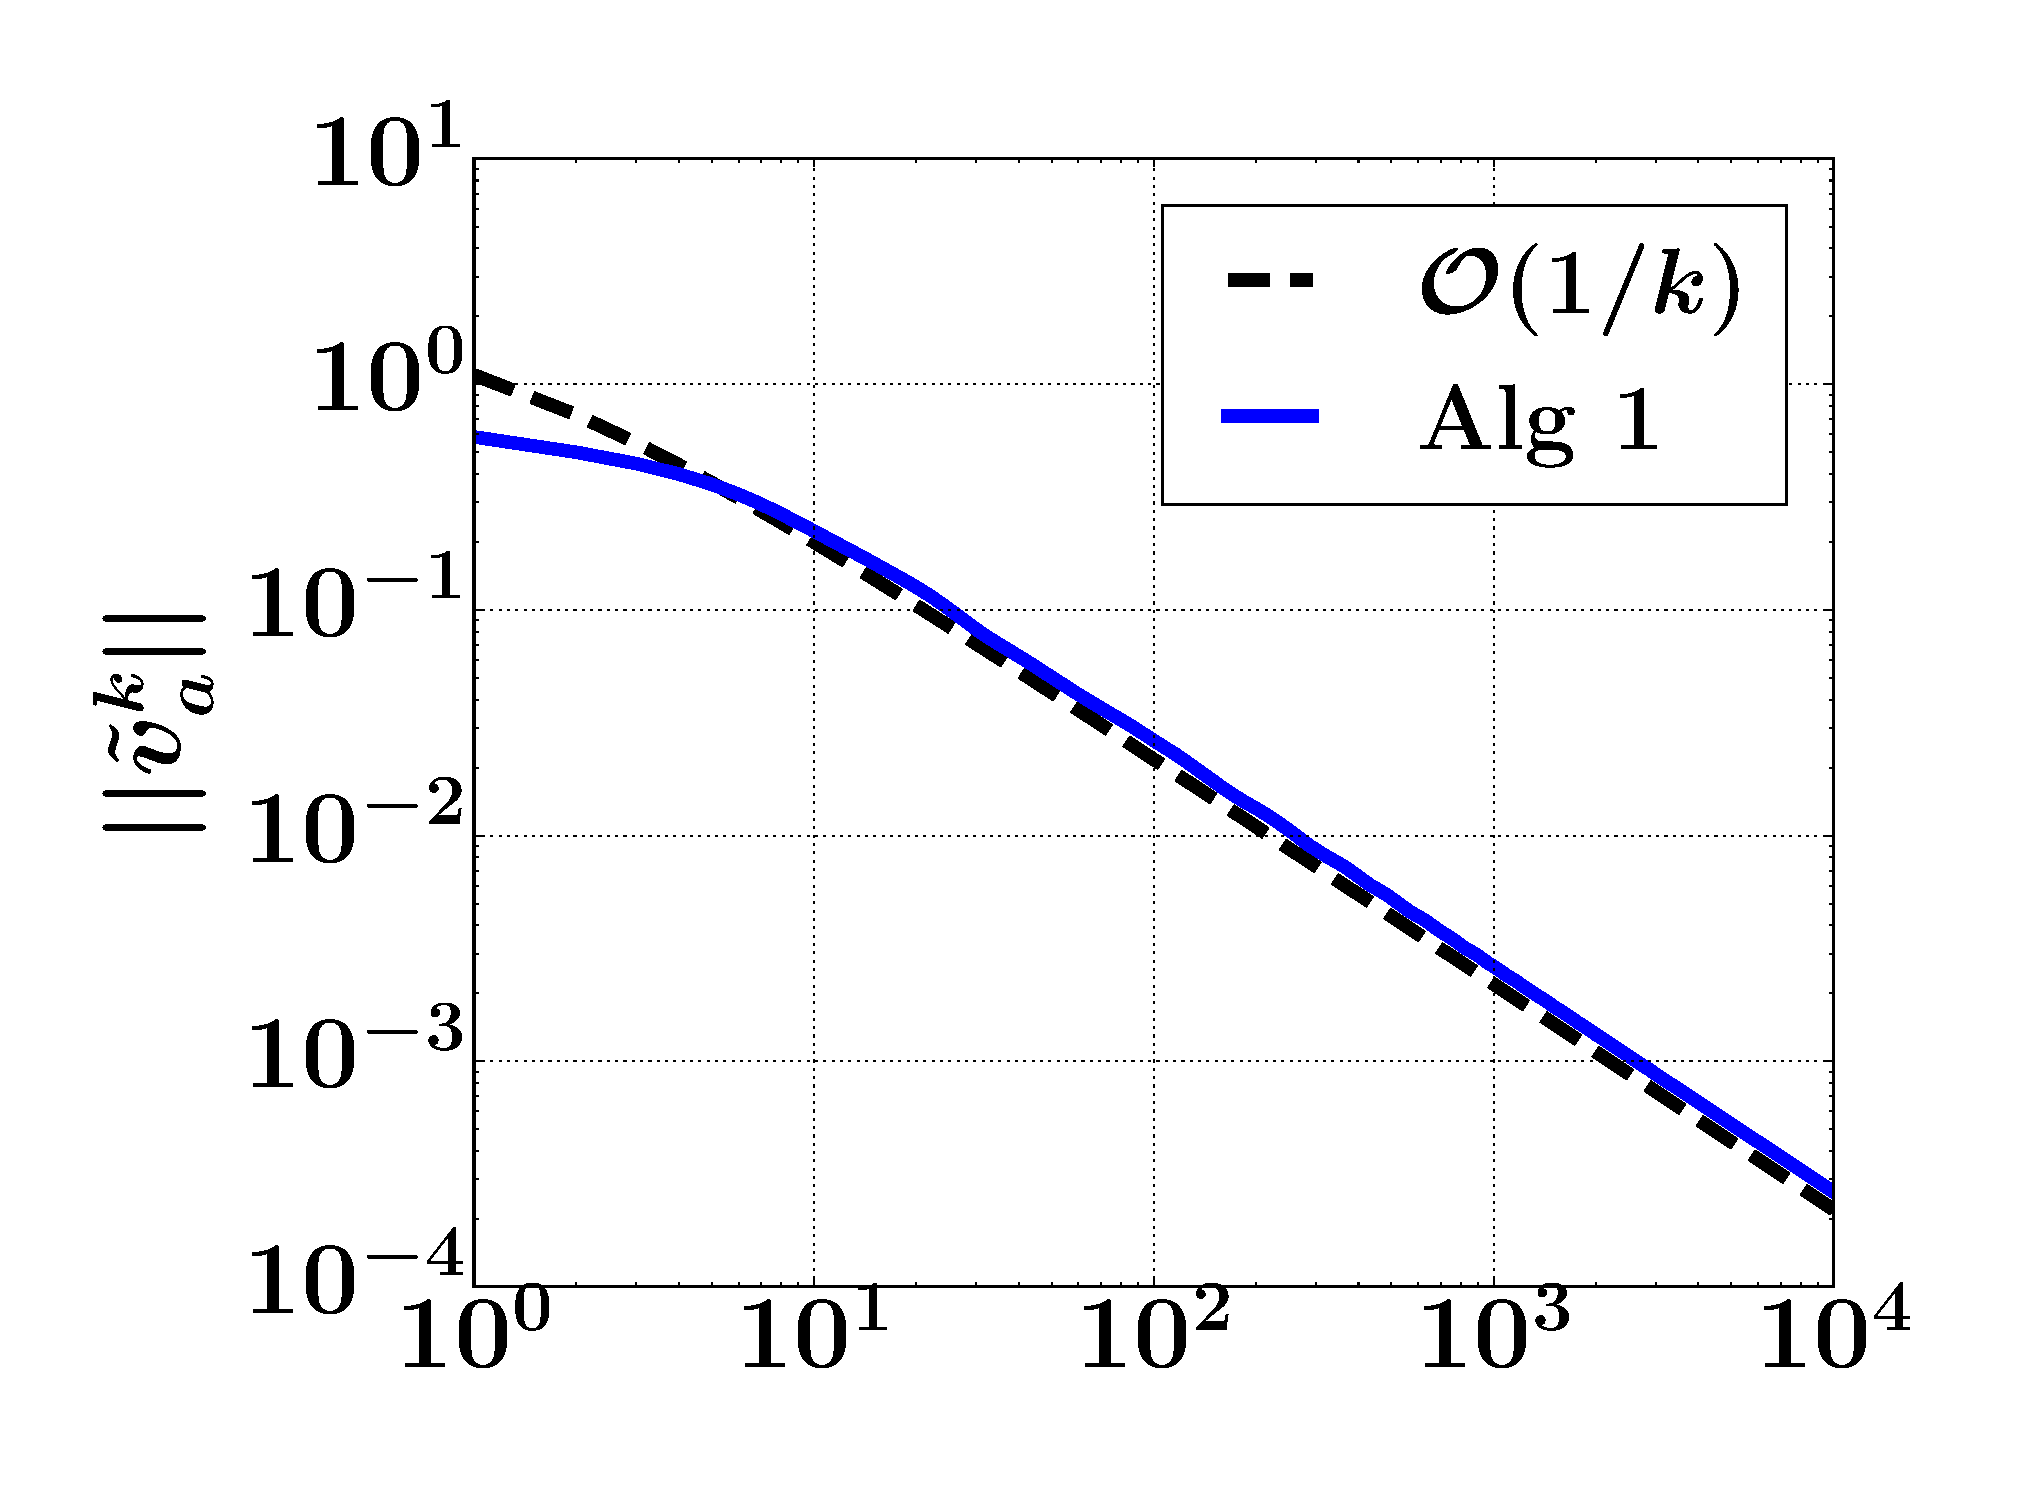
\includegraphics[width=.33\linewidth]{simplex_dgap.pdf}
  }
  \hspace{-2em}
  \subfigure[Toy Poker]{
    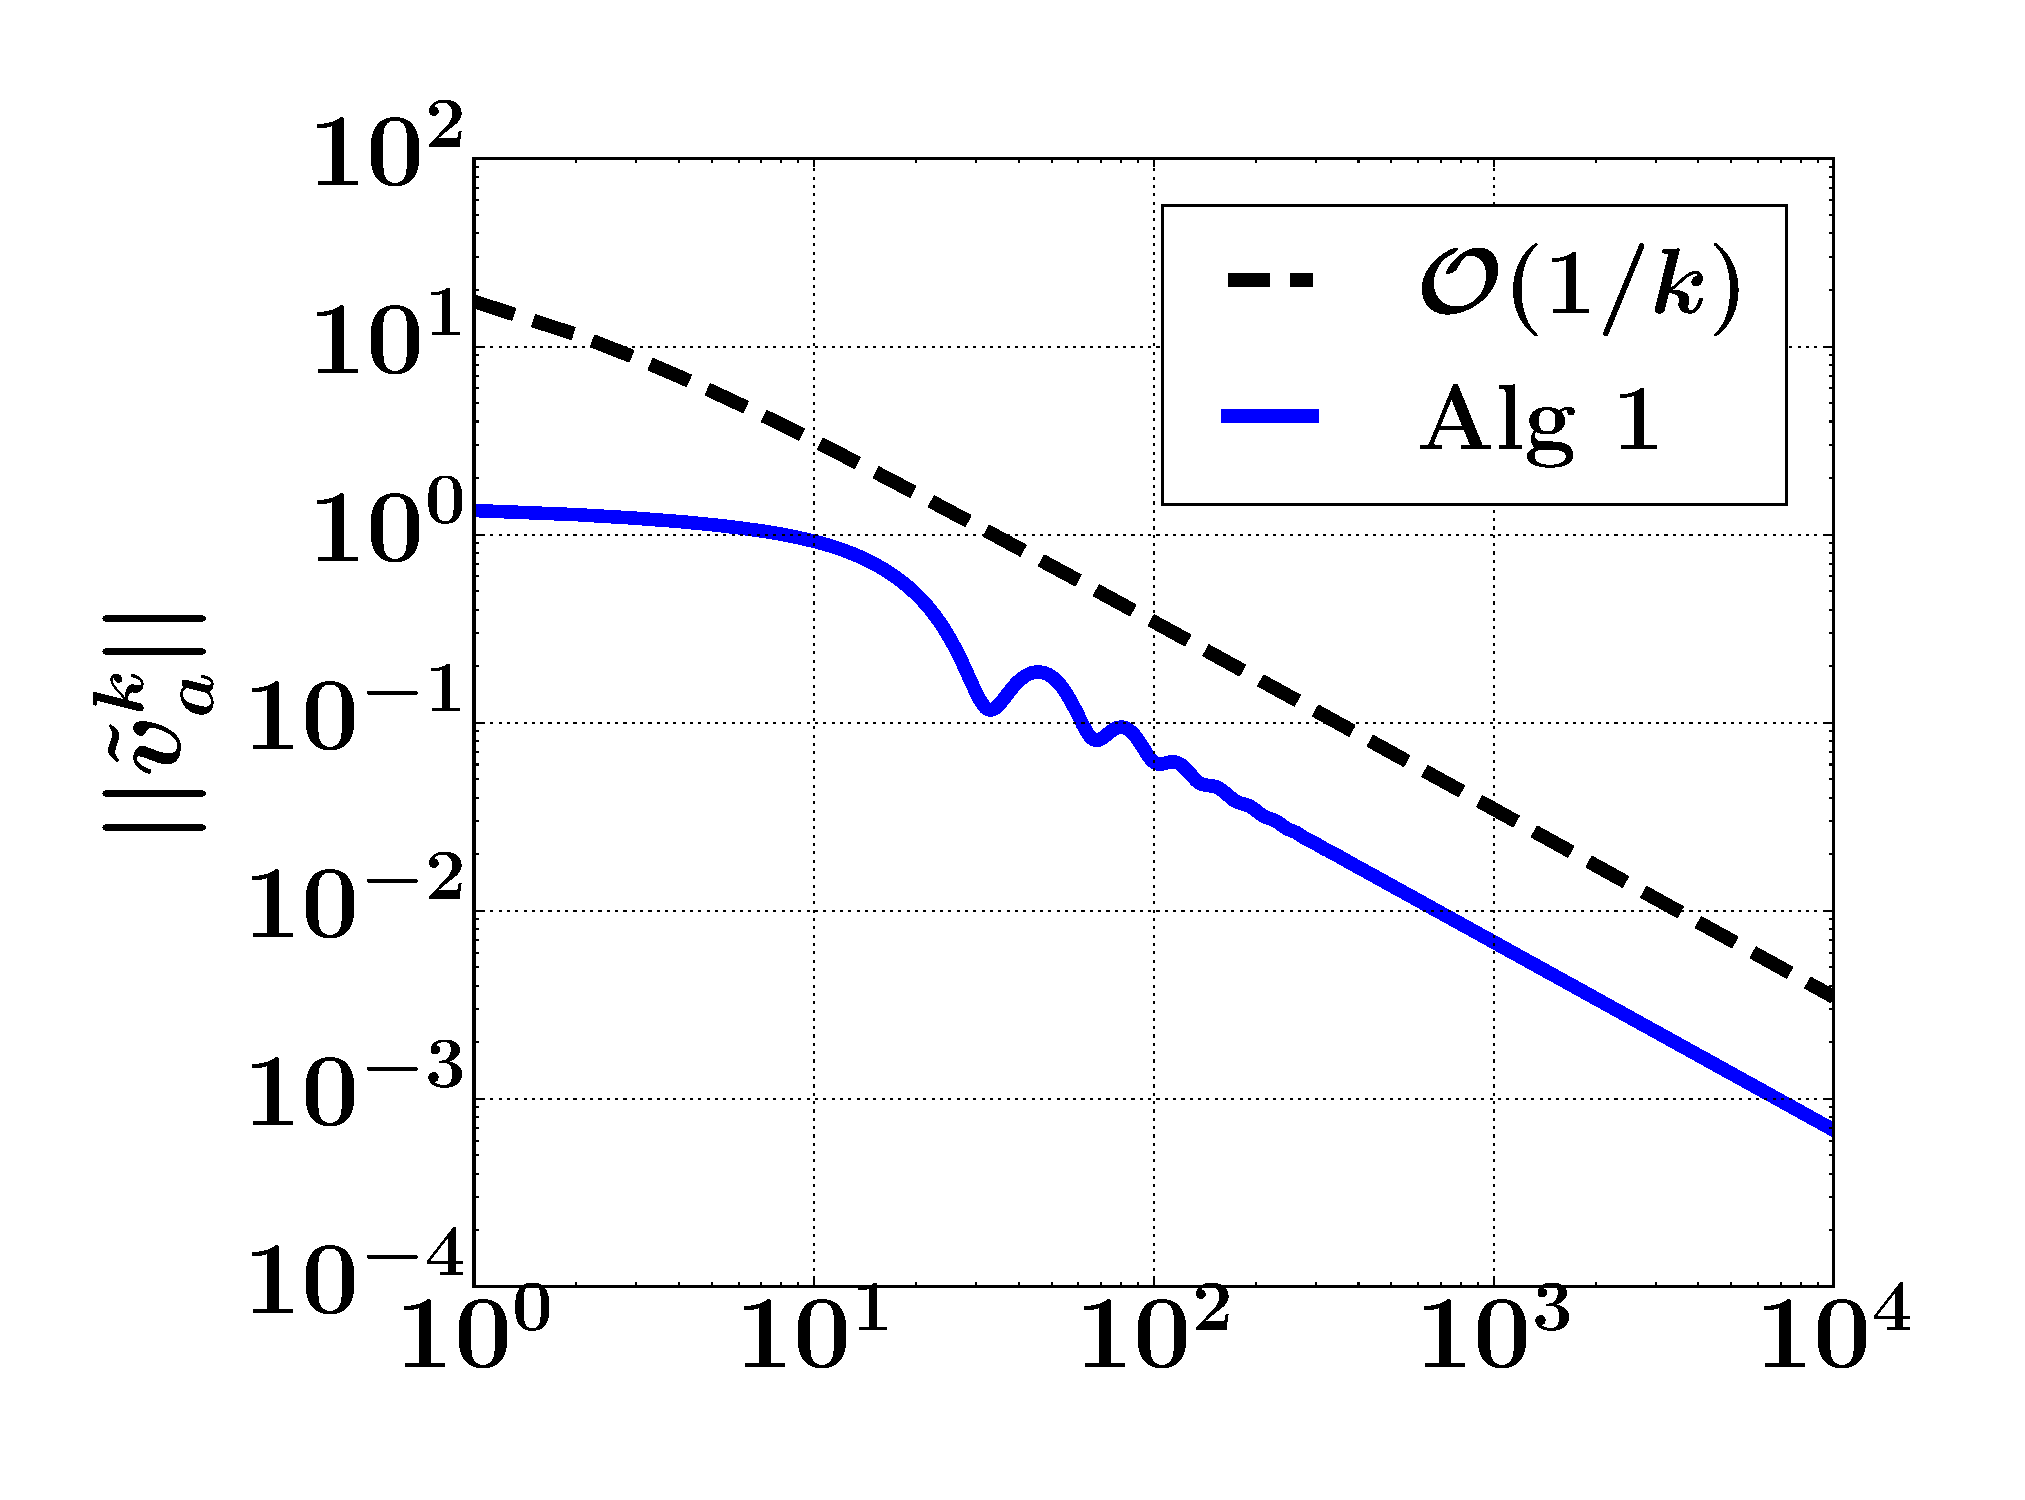
\includegraphics[width=.33\linewidth]{SimplifiedPoker_dgap.pdf}
  }
  \hspace{-2em}
  \subfigure[Kuhn 3-card Poker]{
    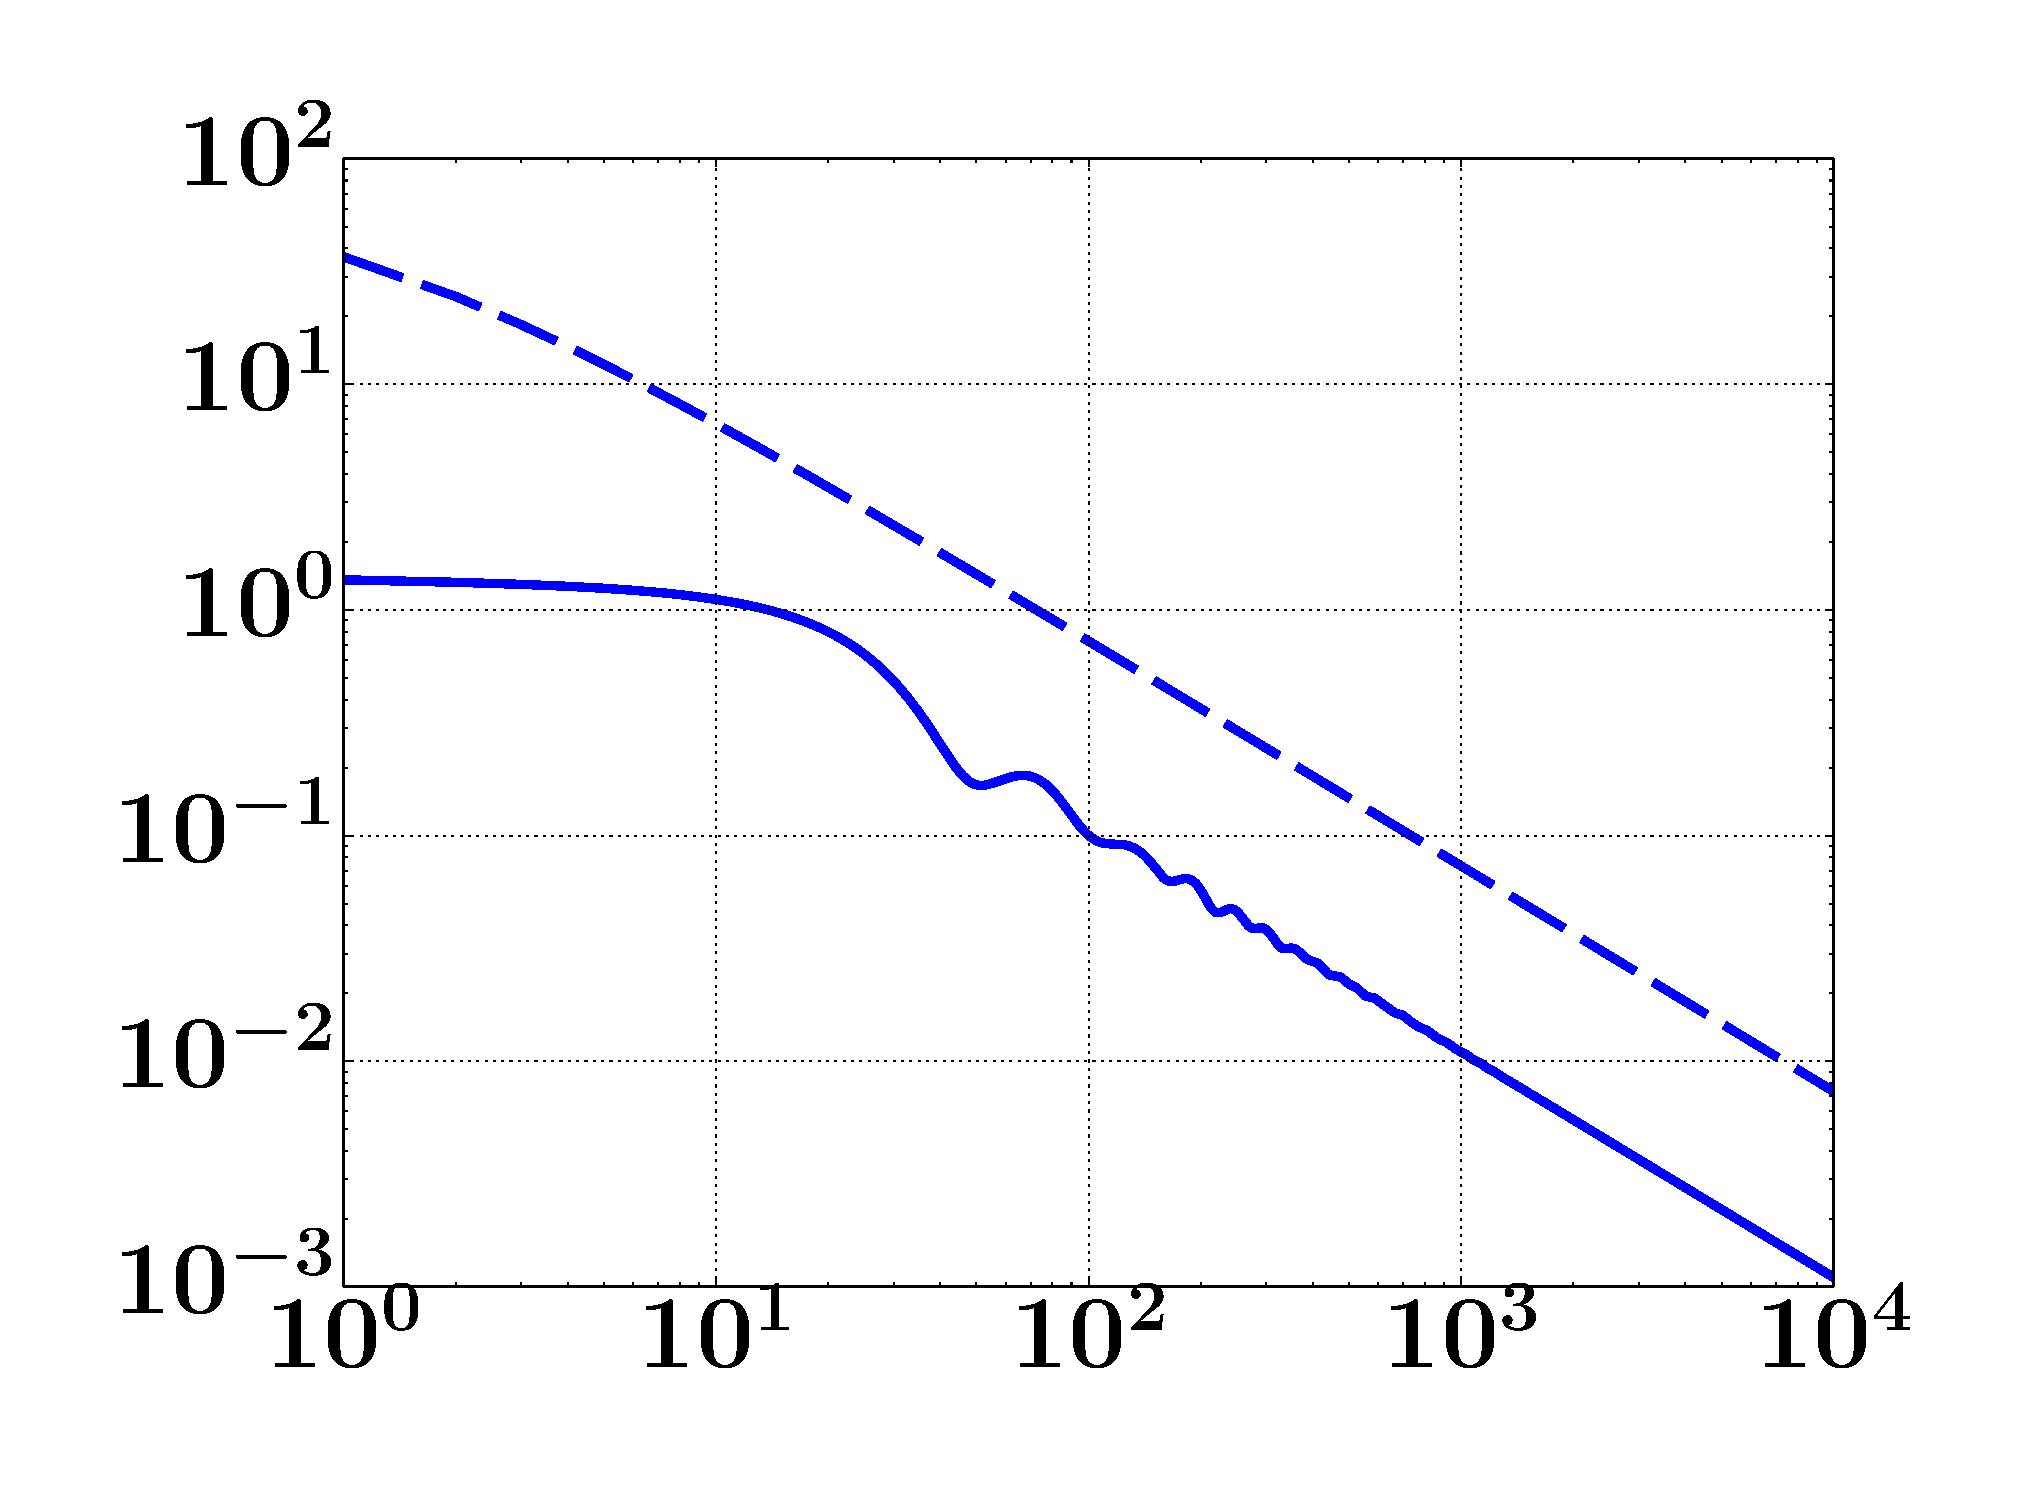
\includegraphics[width=.33\linewidth]{Kuhn3112_dgap.pdf}
  }
  \vspace{-1em}
  \hspace{-1em}
  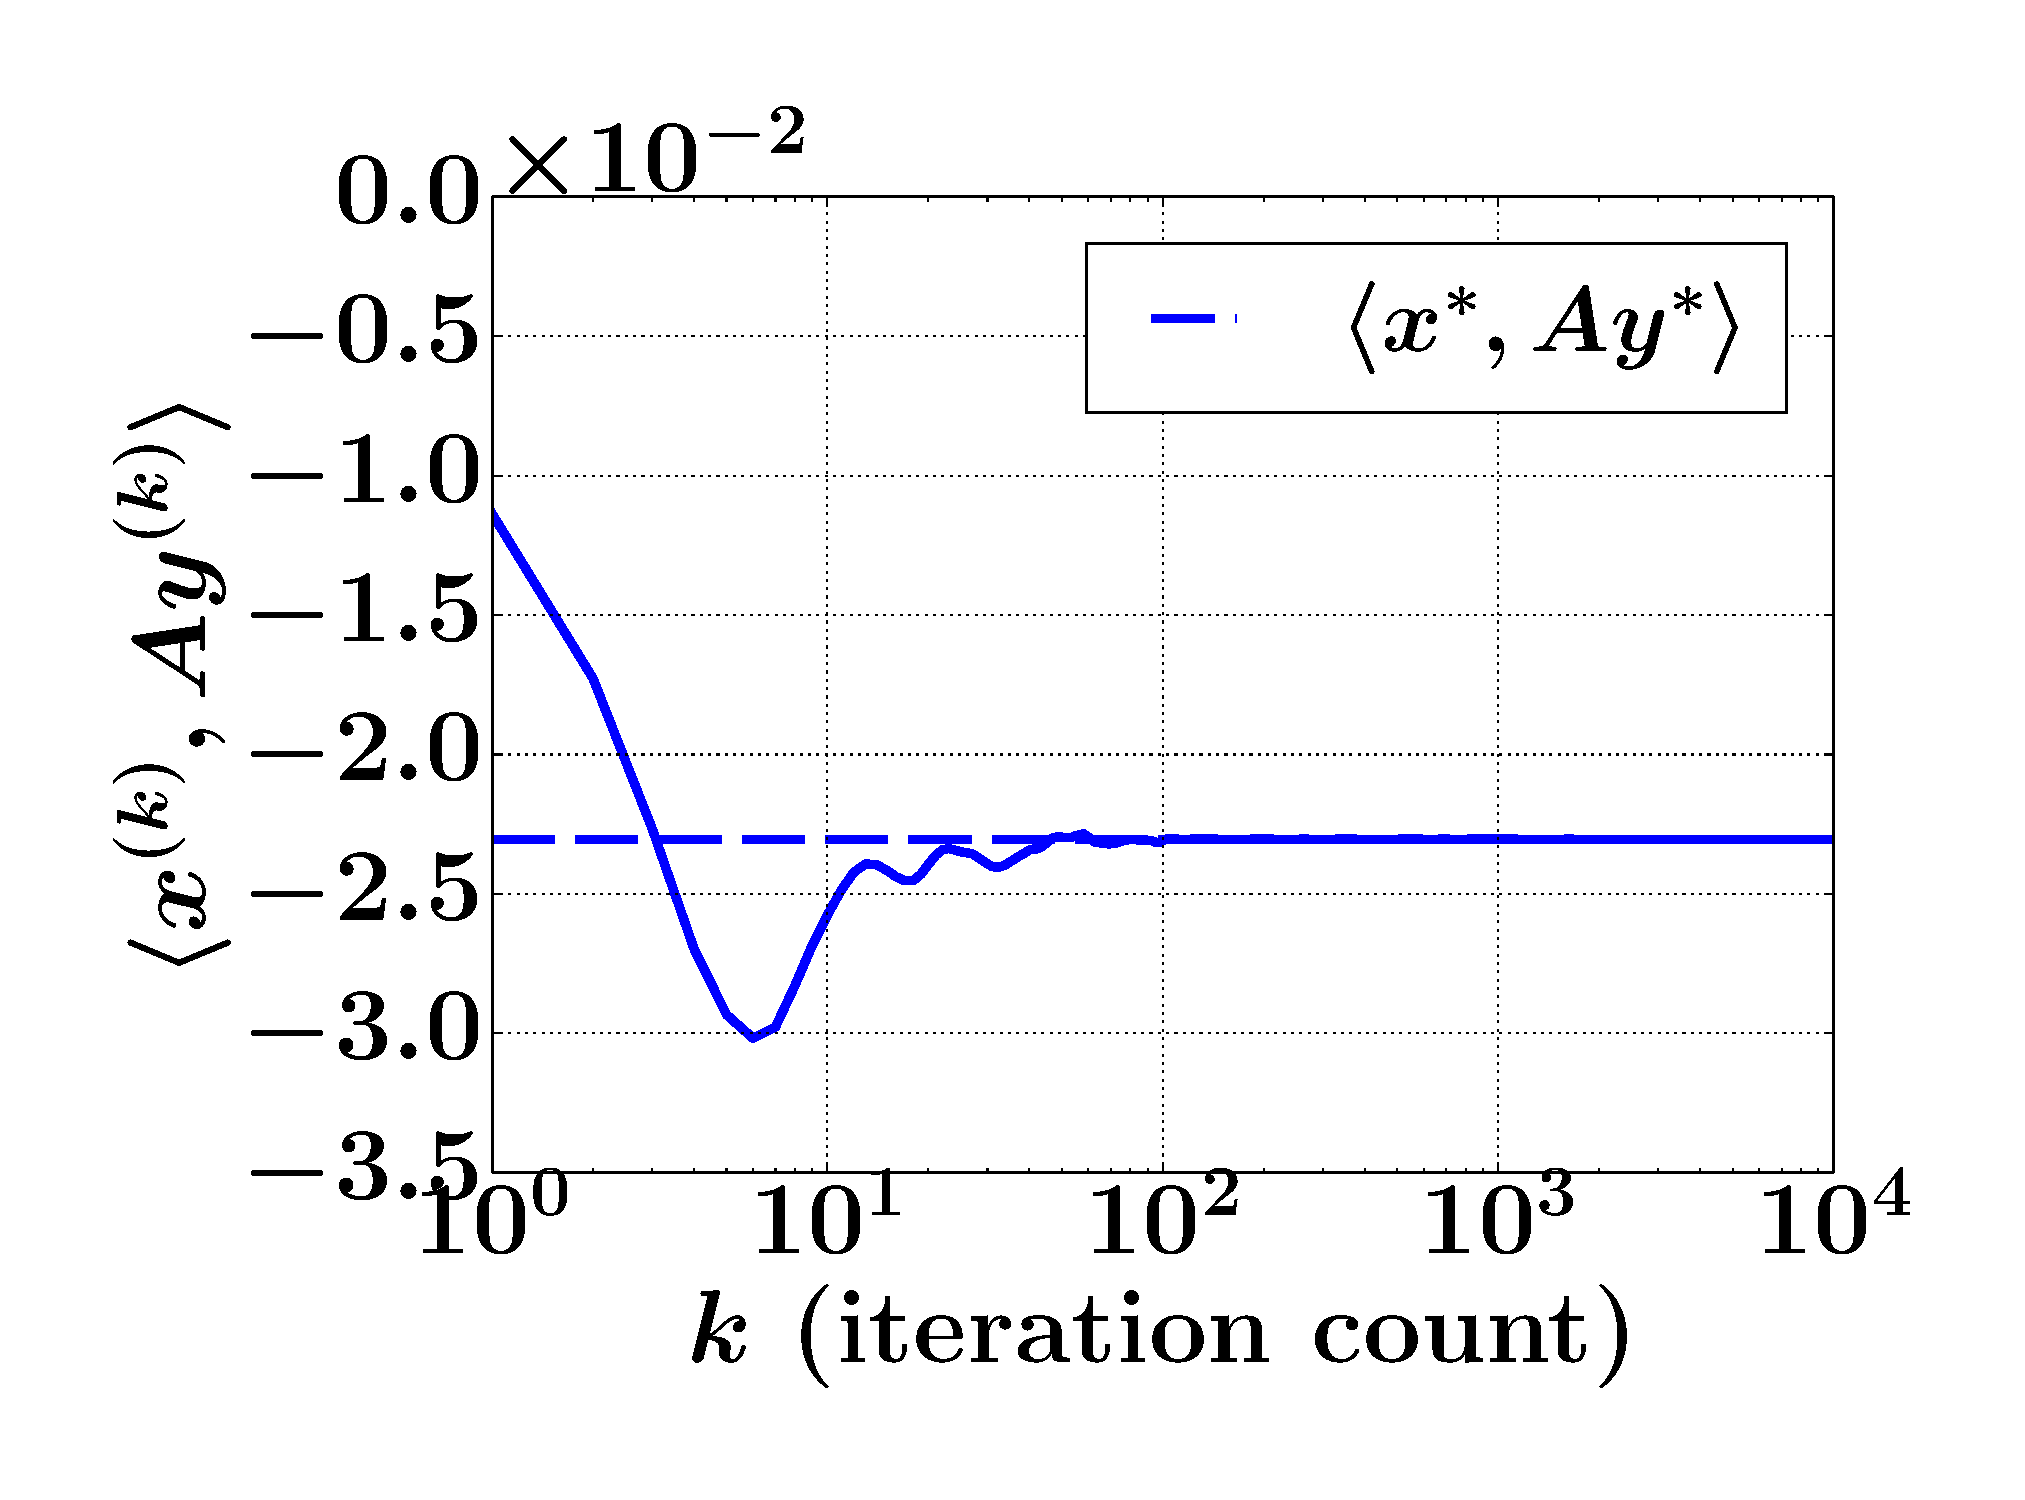
\includegraphics[width=.34\linewidth]{simplex_NE.pdf}
  \hspace{-1em}
  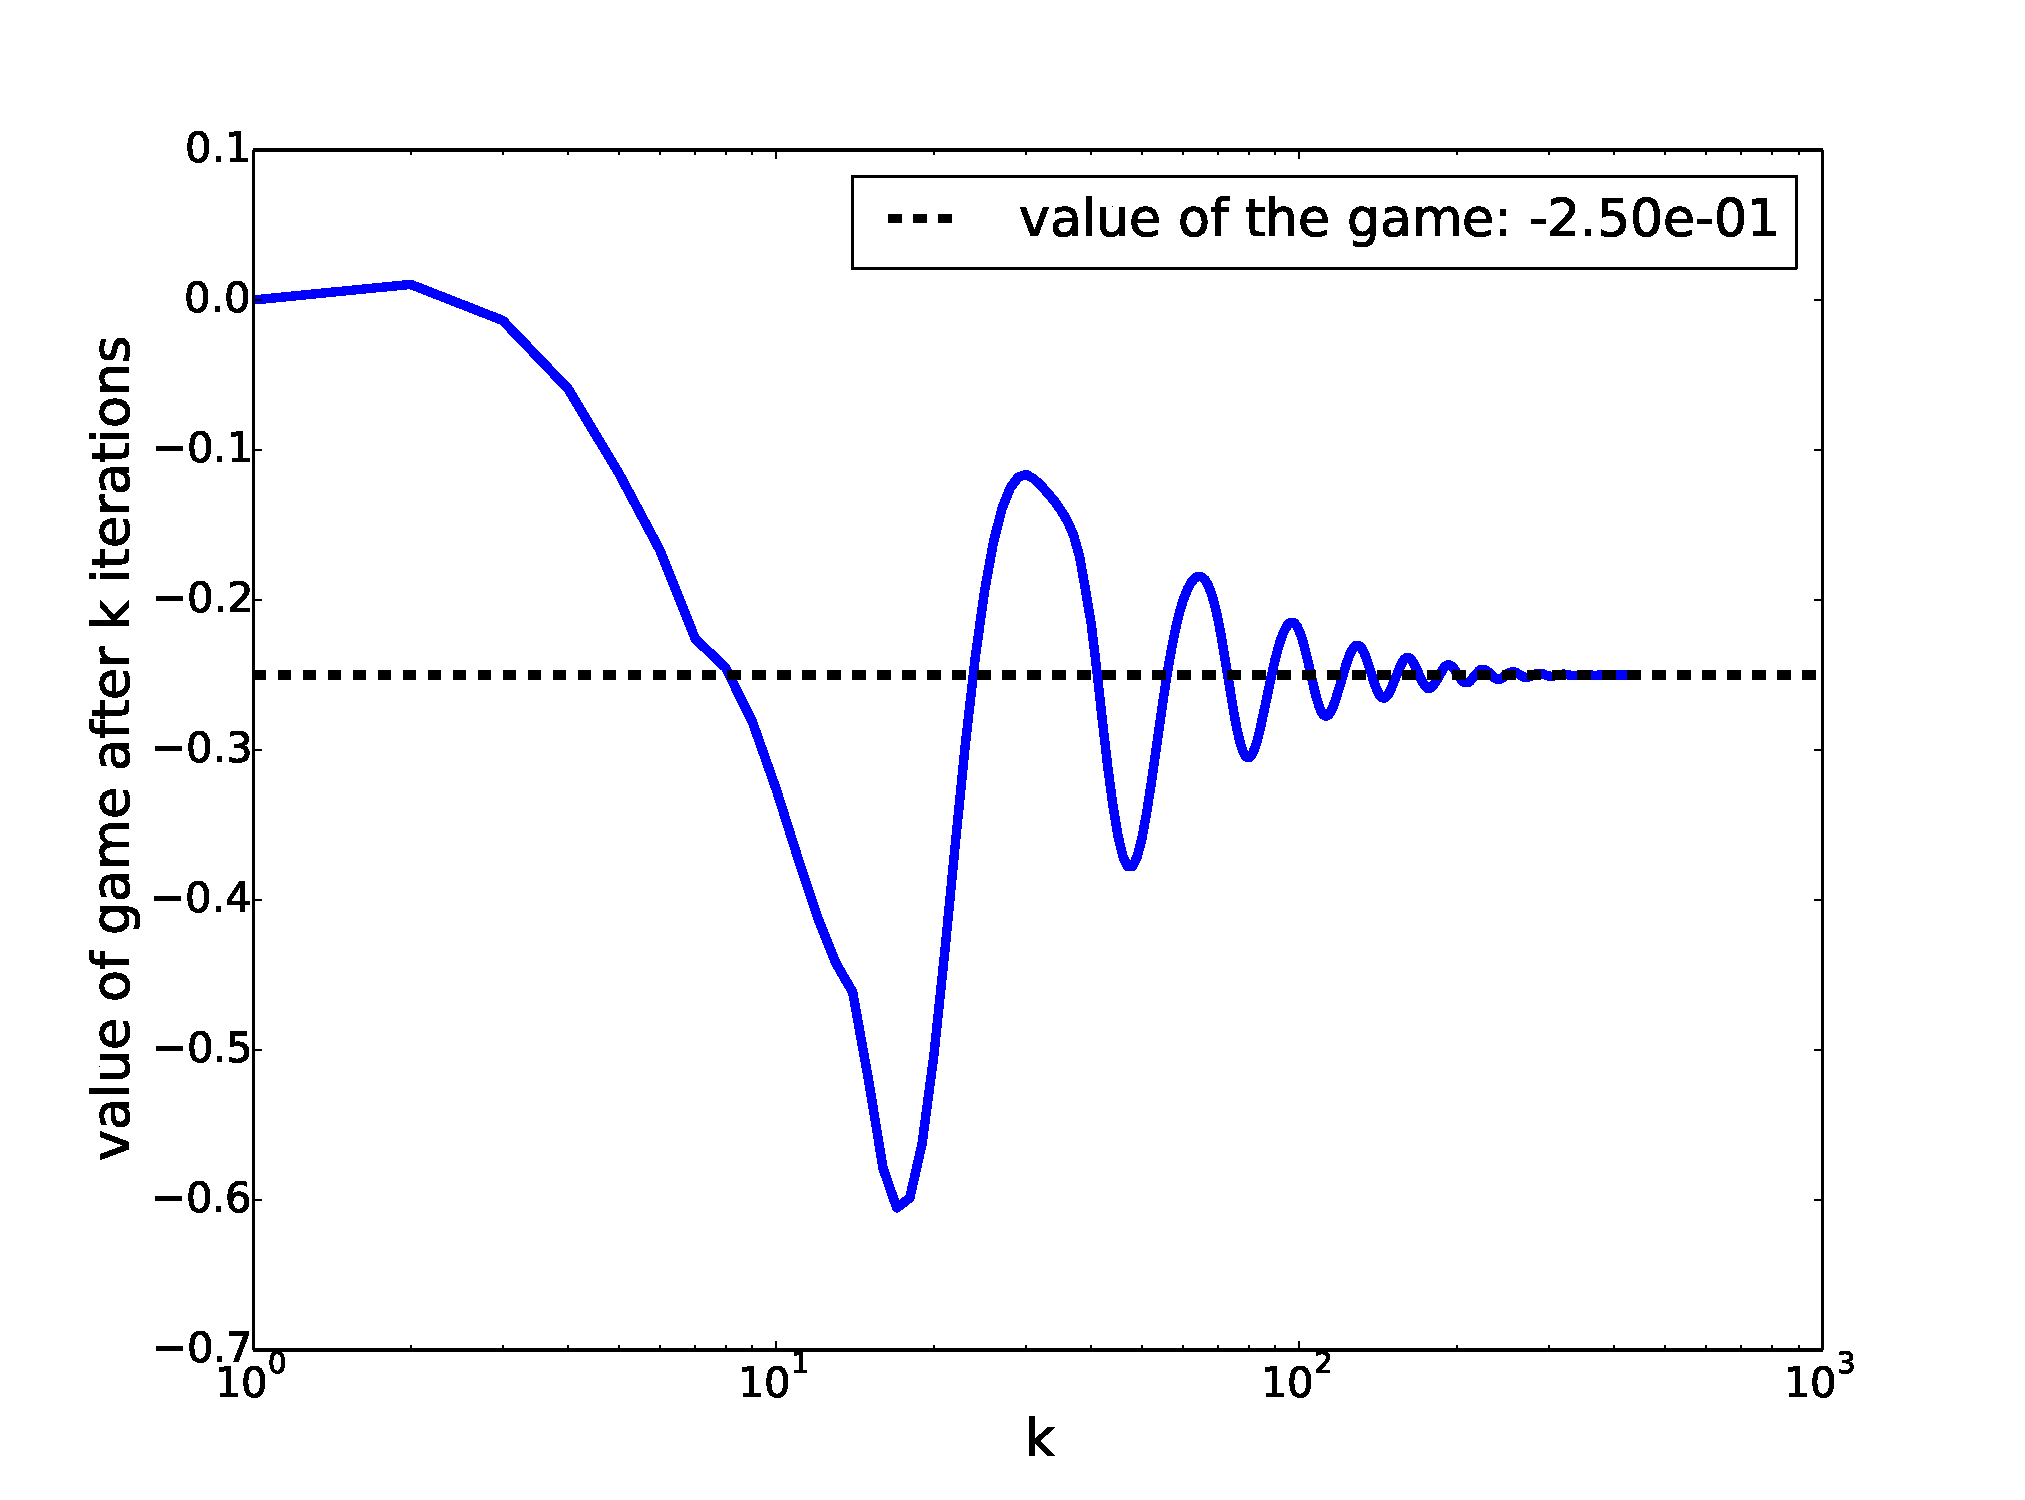
\includegraphics[width=.33\linewidth]{SimplifiedPoker_NE.pdf}
  \hspace{-1em}
  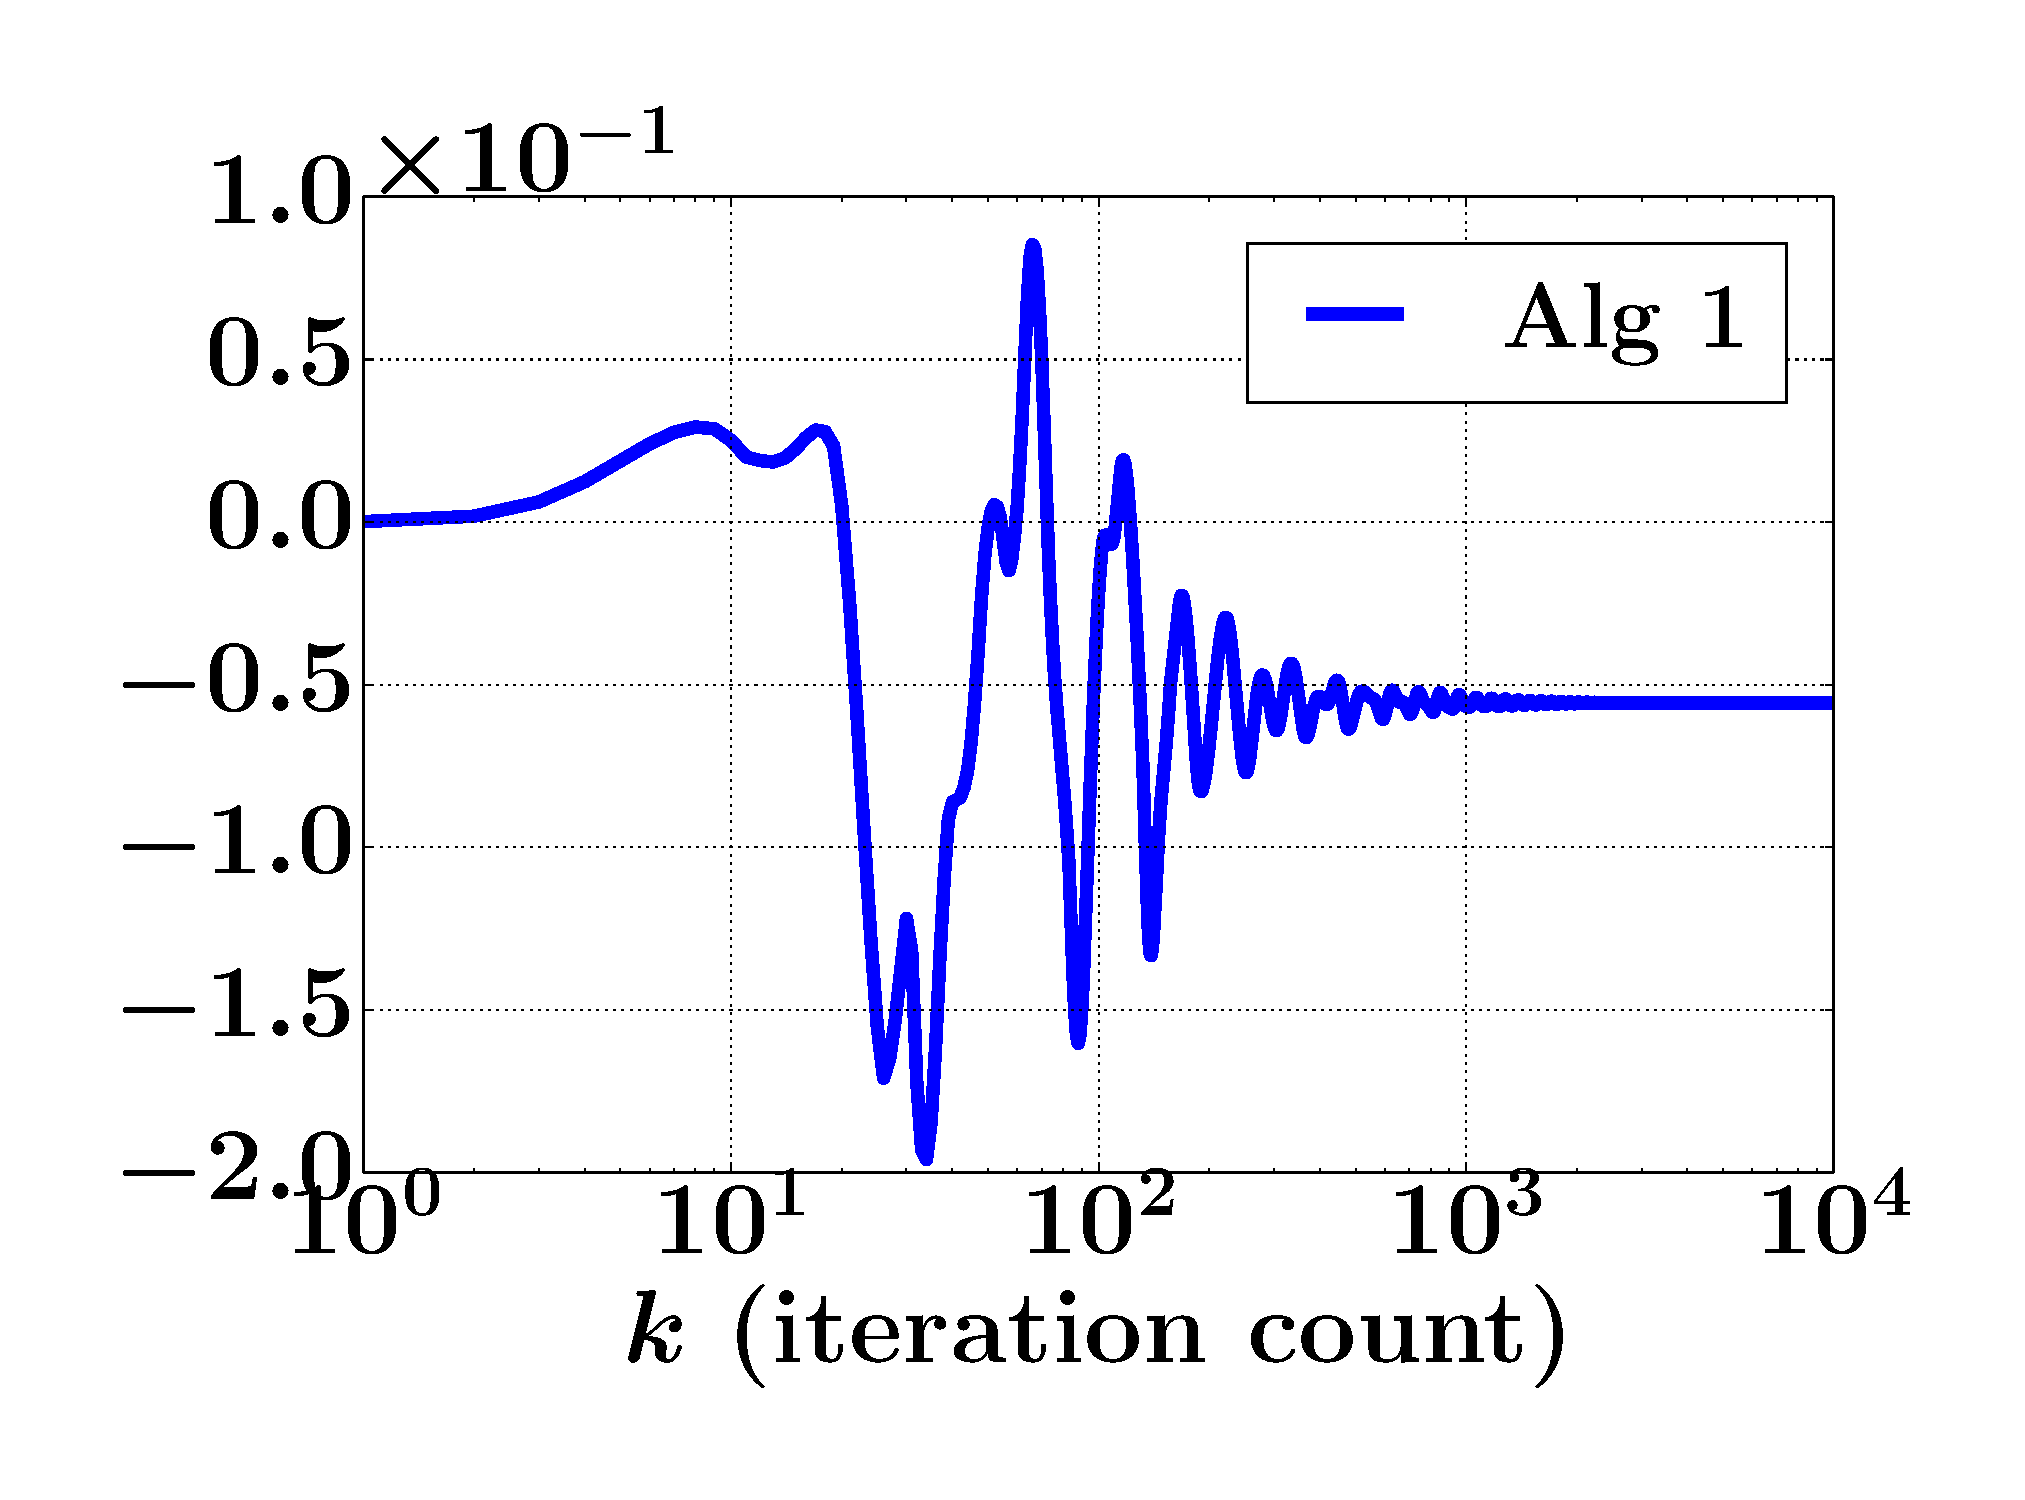
\includegraphics[width=.33\linewidth]{Kuhn3112_NE.pdf}
  \caption{Convergence curves of Algorithm
    \ref{Tab:algo}. \textbf{Top row}: Evolution of ergodic
    primal-dual gap. \textbf{Bottom row}: Evolution of
    value of game.}
  \label{Tab:dgap_curve}
\end{figure}

\paragraph{\textbf{Matrix game on simplexes.}}
Any matrix $A \in \mathbb{R}^{n_1 \times n_2}$ specifies a
\textit{matrix game}. The strategy profile of player $k$ is a simplex;
this simplex can be written in the form \eqref{eq:polyhedron} by
taking $E_k := [1, 1, ..., 1] \in \mathbb{R}^{1 \times n_k}$ and $e_k
= 1$. Thus every matrix game on simplexes can be seen as a sequential
game. Now, as in \textbf{nesterov, c-p, etc.}, we generate a $1000
\times 1000$ random matrix whose entries are uniformly identically
distributed in the closed interval $[-1, 1]$.

\paragraph{\textbf{Toy Poker game.}}
The sequence-form representation for this Toy Poker game is given by
(showing only nonzero entries):\\

$E_1 \in \mathbb{E}^{3 \times 5}$ with $E_1(0,0) = E_1(1,1) =
E_1(1,2) = E_1(2,3) = E_1(2,4) = \textbf{1}$,
$E_1(1,0) = E_1(2,0) = \textbf{-1}$; \\

$E_2 \in \mathbb{E}^{3 \times 5}$ with $E_2(0,0) = E_2(1,1) = E_2(1,2)
= E_2(2,3) = E_2(2,4) = \textbf{1}$, $E_2(1,0) = E_2(2,0) =
\textbf{-1}$; and \\

$A \in \mathbb{E}^{5 \times 5}$ with $A(2,0) =
A(4,0) = \textbf{-0.5}$, $A(1,3) = \textbf{1}$, $A(3,1) =
\textbf{-1}$, $A(1,2) = A(1,4) = A(3,2) = A(3,4) = \textbf{0.25}$.


\paragraph{\textbf{Kuhn 3-card Poker.}}
The game has $n_1 = n_2 = 13$ and $l_1 = l_2 = 7$, and its
sequence-form is given by:\\

$E_1 \in \mathbb{E}^{7 \times 13}$ with $E_1(0,0) = E_1(1,9) =
E_1(1,12) = E_1(2,1) = E_1(2,4) = E_1(3,5) =
E_1(3,8) = E_1(4,2) = E_1(4,3) = E_1(5,6) = E_1(5,7) = E_1(6,10) =
E_1(6,11) = \textbf{1}$, $E_1(1,0) = E_1(2,0) = E_1(3,0) = E_1(4,1) =
E_1(5,5) = E_1(6,9) = \textbf{-1}$; \\

 $E_2 \in \mathbb{E}^{7 \times 13}$
$E_2(0,0) = E_2(1,7) = E_2(1,8) = E_2(2,9) = E_2(2,10) = E_2(3,5) =
E_2(3,6) = E_2(4,11) = E_2(4,12) = E_2(5,1) = E_2(5,2) = E_2(6,3) =
E_2(6,4) = \textbf{1}$, $E_2(1,0) = E_2(2,0) = E_2(3,0) = E_2(4,0) =
E_2(5,0) = E_2(6,0) = \textbf{-1}$; and \\

 $A \in \mathbb{E}^{13 \times
  13}$ with $A(3,8) = A(3,12) = A(4,6) = A(4,10) = A(7,12) = A(8,10) =
\textbf{-0.333333}$, $A(1,7) = A(1,11) = A(2,8) = A(2,12) = A(5,11) =
A(6,4) = A(6,12) = A(10,4) = A(10,8) = \textbf{-0.166667}$, $A(7,4) =
A(8,2) = A(11,4) = A(11,8) = A(12,2) = A(12,6) = \textbf{0.333333}$,
$A(4,5) = A(4,9) = A(5,3) = A(8,1) = A(8,9) = A(9,3) = A(9,7) =
A(12,1) = A(12,5) = \textbf{0.166667}$.\\

The pair $(x^*, y^*) \in \mathbb{R}^{13} \times \mathbb{R}^{13}$ of
realization plans given by

\begin{eqnarray*}
  \begin{split}
    x^* &= [1, 0.759, 0.759, 0, 0.241, 1, 0.425, 0.575, 0, 0.275, 0,
      0.275, 0.725]^T,\\
    y^* &= [1, 1, 0, 0.667, 0.333, 0.667, 0.333, 1, 0, 0, 1, 0, 1]^T
    \end{split}
\end{eqnarray*}
is a Nash $10^{-4}$-equlibrium computed in 1500 iterations of
Algorithm  \ref{Tab:algo}. The convergence curves are shown
in Fig \ref{Tab:dgap_curve}. One easy checks that this equilibrium is
feasible. Indeed,

\begin{eqnarray*}
  \begin{split}
    E_1x^* - e_1 = [&4.76 \times 10^{-5}, -1.91 \times 10^{-5}, 5.67
      \times 10^{-5}, 8.23 \times 10^{-6}, 2.90 \times 10^{-5}, \\&
      -8.62 \times 10^{-7}, -1.96 \times 10^{-5}]^T
    \end{split}
\end{eqnarray*}
and

\begin{eqnarray*}
  \begin{split}
    E_2y^* - e_2 = [&-7.04 \times 10^{-7}, 2.27 \times 10^{-6}, -3.29
      \times 10^{-6}, -1.50 \times 10^{-6},\\
      &2.92 \times 10^{-6}, -4.97 \times 10^{-7}, -5.85 \times
      10^{-7}]^T
    \end{split}
\end{eqnarray*}
Finally, one checks that
\begin{eqnarray*}
  {x^*}^TAy^* = \textbf{-0.05555},
\end{eqnarray*}
 which agrees to 5 d.p with the value of $-1 / 18$ computed
 analytically by H. W. Kuhn in his 1950 paper \cite{kuhn}. The
 evolution of the dual gap and the expected value of the game across
 iterations is shown in Figure \ref{Tab:dgap_curve}.


\section{Conclusion}
Making use of the sequence-form representation
\cite{koller1992complexity,von1996efficient,vonequilibrium}, we have
deviced a primal-dual algorithm for computing Nash equilibria in
two-person zero-sum sequential games with imcomplete information (like
Texas Hold'em, etc.). Our algorithm is simple to implement, with a
very low constant cost per iteration, and enjoys a rigorous
convergence theory with a proven $\mathcal{O}(1/min(\rho,\epsilon))$ convergence
in terms of basic operations (matvec products, clipping, etc.), to a
Nash $(\rho,\epsilon$-equilibrium of the game.

Equilibrium problems are saddle-point convex-concave problems, and as
such a natural choice for an algorithm would be in the family of
primal-dual algorithms. The author believes such primal-dual schemes
will receive more attention in the algorithmic game theory community
in future.


\medskip \noindent
%% \paragraph{About the author:} I'm a first-year PhD student in Computer Science at Universit\'e de Parix XI. My thesis focuses on novel techniques for optimization on Lie groups (of diffeomorphisms), and other structured manifolds, the aim being to obtain better algorithms for nonlinear registration of fMRI brain images and enhance the charting of human functional connectomes.

\small
\bibliographystyle{llcns2e/splncs03}
\bibliography{bib}

\end{document}
